\documentclass[]{article}
\usepackage{siunitx}
\usepackage{hyperref}
\usepackage{float}
\usepackage{graphicx}
\usepackage{dcolumn}
\usepackage[english]{babel}
\usepackage{csvsimple}
\usepackage{listings}
\usepackage{longtable}

\DeclareSIUnit\jansky{jy}
\DeclareSIUnit\pc{pc}
\DeclareSIUnit\solarlum{L_\odot}

%opening
\title{Lab 6}
\author{Miles Lucas}
\date{\today}
\begin{document}

\maketitle

\section{IRAS Sources around KR 140}

Output table from ds9 searching around $ 2^h 20^m 12.589^s $ \ang{+61;06;03.255} within a \SI{15}{\arcminute} rectangle filtered for IRAS sources.

\csvreader[
centered tabular=rrl, 
table head=\hline RA ($\deg$) & DEC ($\deg$) & Main ID \\ \hline\hline, 
table foot=\hline]
{../data/iras.csv}{}{\csvcoliv & \csvcolv & \csvcoliii}

The IDs of these sources were then used in a VizieR query of the IRAS catalogue of Point Sources, Version 2.0 (IPAC 1986).

\begin{lstlisting}[language=SQL,basicstyle=\footnotesize,frame=single,]
	-- output format : csv
	SELECT "II/125/main".IRAS,  
	"II/125/main".RA1950,  
	"II/125/main".DE1950,  
	"II/125/main".Fnu_12,  
	"II/125/main".e_Fnu_12,  
	"II/125/main".Fnu_25,
	"II/125/main".e_Fnu_25,  
	"II/125/main".Fnu_60,  
	"II/125/main".e_Fnu_60,  
	"II/125/main".Fnu_100,  
	"II/125/main".e_Fnu_100  
	FROM "II/125/main"
	WHERE "II/125/main".IRAS LIKE '02156+6045' OR
	"II/125/main".IRAS LIKE '02157+6053' OR
	"II/125/main".IRAS LIKE '02160+6057' OR
	"II/125/main".IRAS LIKE '02165+6053' OR
	"II/125/main".IRAS LIKE '02168+6052' OR
	"II/125/main".IRAS LIKE '02171+6058' OR
	"II/125/main".IRAS LIKE '02174+6052'
\end{lstlisting}

From this query the following table was created. Note the errors are whole number percentage errors (ie 25 means 25\% error on the given measurement)

\csvreader[
centered tabular=llrrrrrrrrrr, 
table head=\hline IRAS & $F_{\nu,12}$ & $\epsilon_{F_{\nu,12}}$ & $F_{\nu,25}$ & $\epsilon_{F_{\nu,25}}$ & $F_{\nu,60}$ & $\epsilon_{F_{\nu,60}}$ &  $F_{\nu,100}$ & $\epsilon_{F_{\nu,100}}$ \\ \hline\hline, 
table foot=\hline]
{../data/result.csv}{}{\csvcoli & \csvcoliv & \csvcolv & \csvcolvi & \csvcolvii & \csvcolviii & \csvcolix & \csvcolx & \csvcolxi}

From these values I created a color plot, where 

\begin{equation}
x = \log_{10}{\frac{F_{\nu, 60}}{F_{\nu, 100}}}
\end{equation}

\begin{equation}
\sigma_x = \frac{1}{100 \ln{10}}\sqrt{\epsilon_{F_{\nu,60}}^2 + \epsilon_{F_{\nu,100}}^2}
\end{equation}

\begin{equation}
y = \log_{10}{\frac{F_{\nu, 25}}{F_{\nu, 12}}}
\end{equation}

\begin{equation}
\sigma_y = \frac{1}{100 \ln{10}}\sqrt{\epsilon_{F_{\nu,25}}^2 + \epsilon_{F_{\nu,12}}^2}
\end{equation}

\begin{figure}
	\centering
	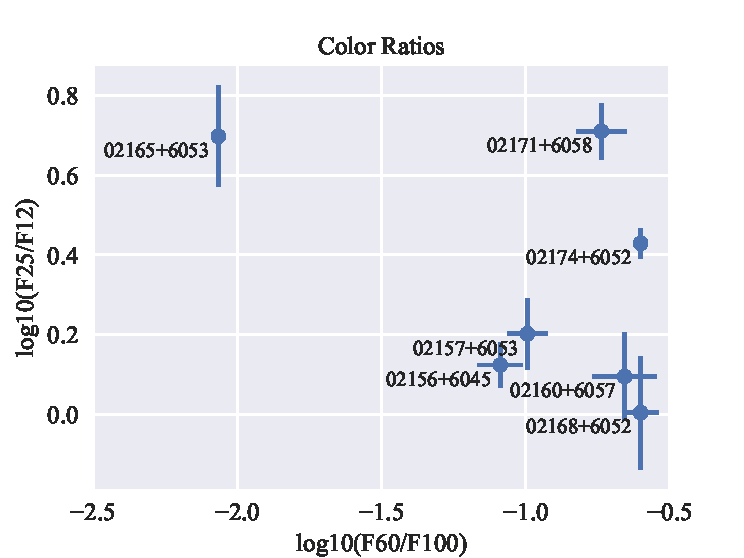
\includegraphics[]{figs/colors.pdf}
\end{figure}

I also made a spectrum plot shown in . Using this, I integrated to find the total infrared flux to be \SI{239}{\jansky}. Using this and an assumed distance of \SI{2.3}{\kilo\pc} I can estimate the integrated flux over the whole star and find its luminosity using \autoref{eqn:lum}. The luminosity I have estimated is \SI{7.50e18}{\watt} or \SI{1.95e-8}{\solarlum}

\begin{equation}
L=4\pi D^2 F
\label{eqn:lum}
\end{equation}

\begin{figure}
	\centering
	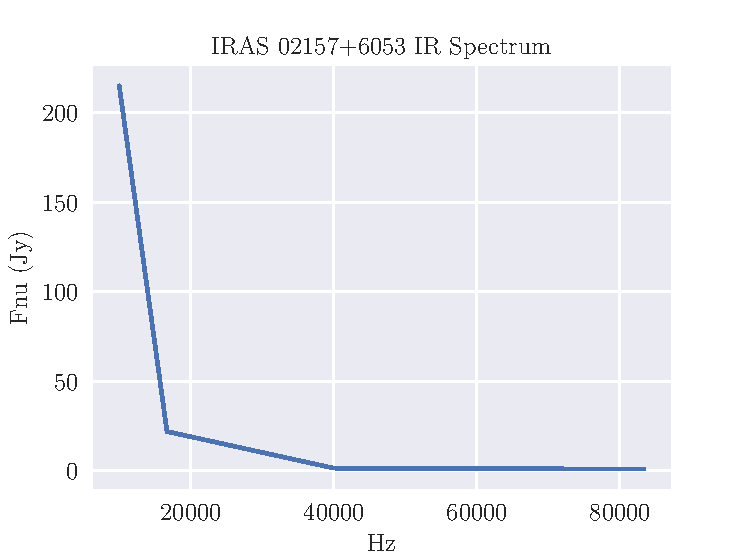
\includegraphics[]{figs/spectrum.pdf}
\end{figure}


\section{KR 140 in the submm}

In the submm photo there is a clump around $i=+133.436, b=-0.022$ that does not correspond with any of the IRAS sources

\section{A 2MASS View of an IRAS Source}

\csvreader[
centered tabular=lllrrrrrr, 
table head=\hline RA & DEC & 2MASS & J & $\epsilon_J$ & H & $\epsilon_H$ & K & $\epsilon_K$ \\ \hline\hline, 
table foot=\hline]
{../data/2mass.csv}{}{\csvlinetotablerow}


\section{Identifying YSOs using 2MASS Data}


\end{document}